%\documentclass[titlepage]{jsarticle}

%\usepackage[dvipdfmx]{graphicx}

%数式用パッケージ
%\usepackage{amsmath, amssymb}
%\usepackage{mathtools}
%\usepackage{cancel}
%\usepackage{cases}
%\usepackage{bm}
%\usepackage{array,booktabs}
%\usepackage{float}

%\usepackage{subcaption}

%ファインマングラフ用パッケージ
%\usepackage{feynmf}



%\graphicspath{{./figure/}}

%\begin{document}

%%%%%%%%%%%%%%%%%%%池満パート開始%%%%%%%%%%%%%%%%%%%

\section{プラスチックシンチレータで取得したデータの解析と結果・考察}
\subsubsection{解析手法}
プラスチックシンチレータ(以下,PS)検出器を用いて取得したデータを以下の方法で解析し,寿命,$g$因子,エネルギー分布を求めた.
\begin{enumerate}
\item イベントディスプレイから,初めの100 ns (50 Sample)の間は信号が来ていないことを確認し,0〜100 ns のデータの平均値をとってそれをbaselineとした.
\item 信号のしきい値(threshold)の決定
\begin{itemize}
\item 宇宙線を用いた予備実験の結果から,12 MeV のエネルギーに対応する信号のピーク値を求めた.
\item そのピーク値から,各チャンネルごとのthreshold値を以下の値に決めた.
\item 寿命測定と$g$因子測定用には,1層目:3 MeV相当,2層目以降:2 MeV相当とした.
\item エネルギー測定用には,1層目:4 MeV相当とし,2層目以降はthresholdを設けなかった.
\end{itemize}
\item 各チャンネルごとで,thresholdを越えた時間を信号の時間(peaktime)とした.
\item イベントディスプレイからおおよその信号の時間幅を決め,信号が検出されてから次の信号を検出するようになるまでのveto時間を40 ns にした.
\item peaktimeから40 ns の間のデータを足すことで信号のchargeを求めた.
\item 寿命と$g$因子について
\begin{itemize}
\item 各層の両側のチャンネルの信号のcoincidenceを取った.ただし,3層目は片側のみの信号である.
\item ここで,coincidenceの条件は,peaktimeが10 ns よりも近いものとした.
\item 寿命測定では,層ごとのcoincidenceをとった.
\item $g$因子測定では,立体角を制限するために,層ごとだけでなくfingerとのcoincidenceを要求した.
\end{itemize}
\item エネルギーについて
\begin{itemize}
\item 予備実験のデータから,各チャンネルごとにキャリブレーションをした.
\item 各層のエネルギーとして,1,2,4層目では両側のチャンネルのエネルギーの平均を取り,3層目では片方のチャンネルのエネルギーを使用した.
\item fingerと1層目の両側のチャンネルの信号のcoincidenceをとり,そのときの全層のエネルギーの和を求めた.
2層目以降のチャンネルで信号がない場合,そのチャンネルのエネルギーは0とした.
\item fingerとのcoincidenceを取ったのは,検出器の中心に入ったe$^{+}$の信号のみを選択し,エネルギー漏れを減らすためである.
\end{itemize}
\end{enumerate}

\subsubsection{信号検出のthreshold値について}
この小節の後で解析の結果を述べるが,その前に,信号検出時のthresholdの値の判断理由について触れておく.

まず,1層目の信号の中には,標的に当たらずにビーム出口から直接検出器に入るミュオンによる信号があると考えた.
1層目のthresholdを他層よりも高く設定しているのは,このようなバックグラウンドを除去するためである.

次に,thresholdの値を1MeV相当にして寿命を求めると,thresholdが高いときよりも長くなった.
よって,1MeV相当のthresholdでは低エネルギーのノイズを信号として処理していると考えた.
一方,寿命測定に関して,thresholdを上げてもfittingの結果は変わらず,統計誤差が大きくなるだけだった.

以上のことを基にして,thresholdの値を判断した.

\subsubsection{得られた崩壊曲線とfittingの結果}
図\ref{lt_layercoin}は,磁場なし標的を用いたときのミュオンの崩壊曲線である.
それを次の$f_{\mathrm{life}}(t)$でfittingした結果が図\ref{lt_layercoin_fit}である
\begin{equation*}
f_{\mathrm{life}}(t) = \exp[-(t+A)/\tau].
\end{equation*}
また,図\ref{g_layercoin}は,磁場あり標的を用いたときのミュオンの崩壊曲線である.
それを次の$f_{g}(t)$でfittingした結果が図\ref{g_layercoin_fit}である.
\begin{equation*}
f_{g}(t) = \exp[-(t+A)/\tau](1+B\cos(\omega t + \delta)).
\end{equation*}

fittigの結果は表\ref{fit_lt},\ref{fit_g}のようになった.表中の誤差はfittingに由来する統計誤差である.

\begin{table}[H]
\caption{寿命$\tau$のfitting結果}
\label{fit_lt}
\begin{center}
\begin{tabular}{cc}\toprule
coincidenceを取った層 	& $\tau$(ns) \\ \midrule
1 			& 2215.0 $\pm$ 9.4 \\
1+2 			& 2212 $\pm$ 12 \\
1+2+3 			& 2196 $\pm$ 16 \\
1+2+3+4 		& 2142 $\pm$ 33 \\ \bottomrule
\end{tabular}
\end{center}
\end{table}%

\begin{table}[H]
\caption{$g$因子のfitting結果}
\label{fit_g}
\begin{center}
\begin{tabular}{ccc}\toprule
coincidenceを取った層 	& $\omega$(/ns) 			& $g$ \\ \midrule
finger+1 		& $( 4.615 \pm 0.016 ) \times 10^{-3}$ 	& 2.0066 $\pm$ 0.0068 \\
finger+1+2 		& $( 4.607 \pm 0.014 ) \times 10^{-3}$ 	& 2.0031 $\pm$ 0.0063 \\
finger+1+2+3 		& $( 4.615 \pm 0.014 ) \times 10^{-3}$ 	& 1.9934 $\pm$ 0.0062 \\
finger+1+2+3+4 		& $( 4.629 \pm 0.023 ) \times 10^{-3}$ 	& 2.0129 $\pm$ 0.0098 \\ \bottomrule
\end{tabular}
\end{center}
\end{table}%


\begin{figure}[H]
\centering
\begin{subfigure}{\columnwidth}
\centering
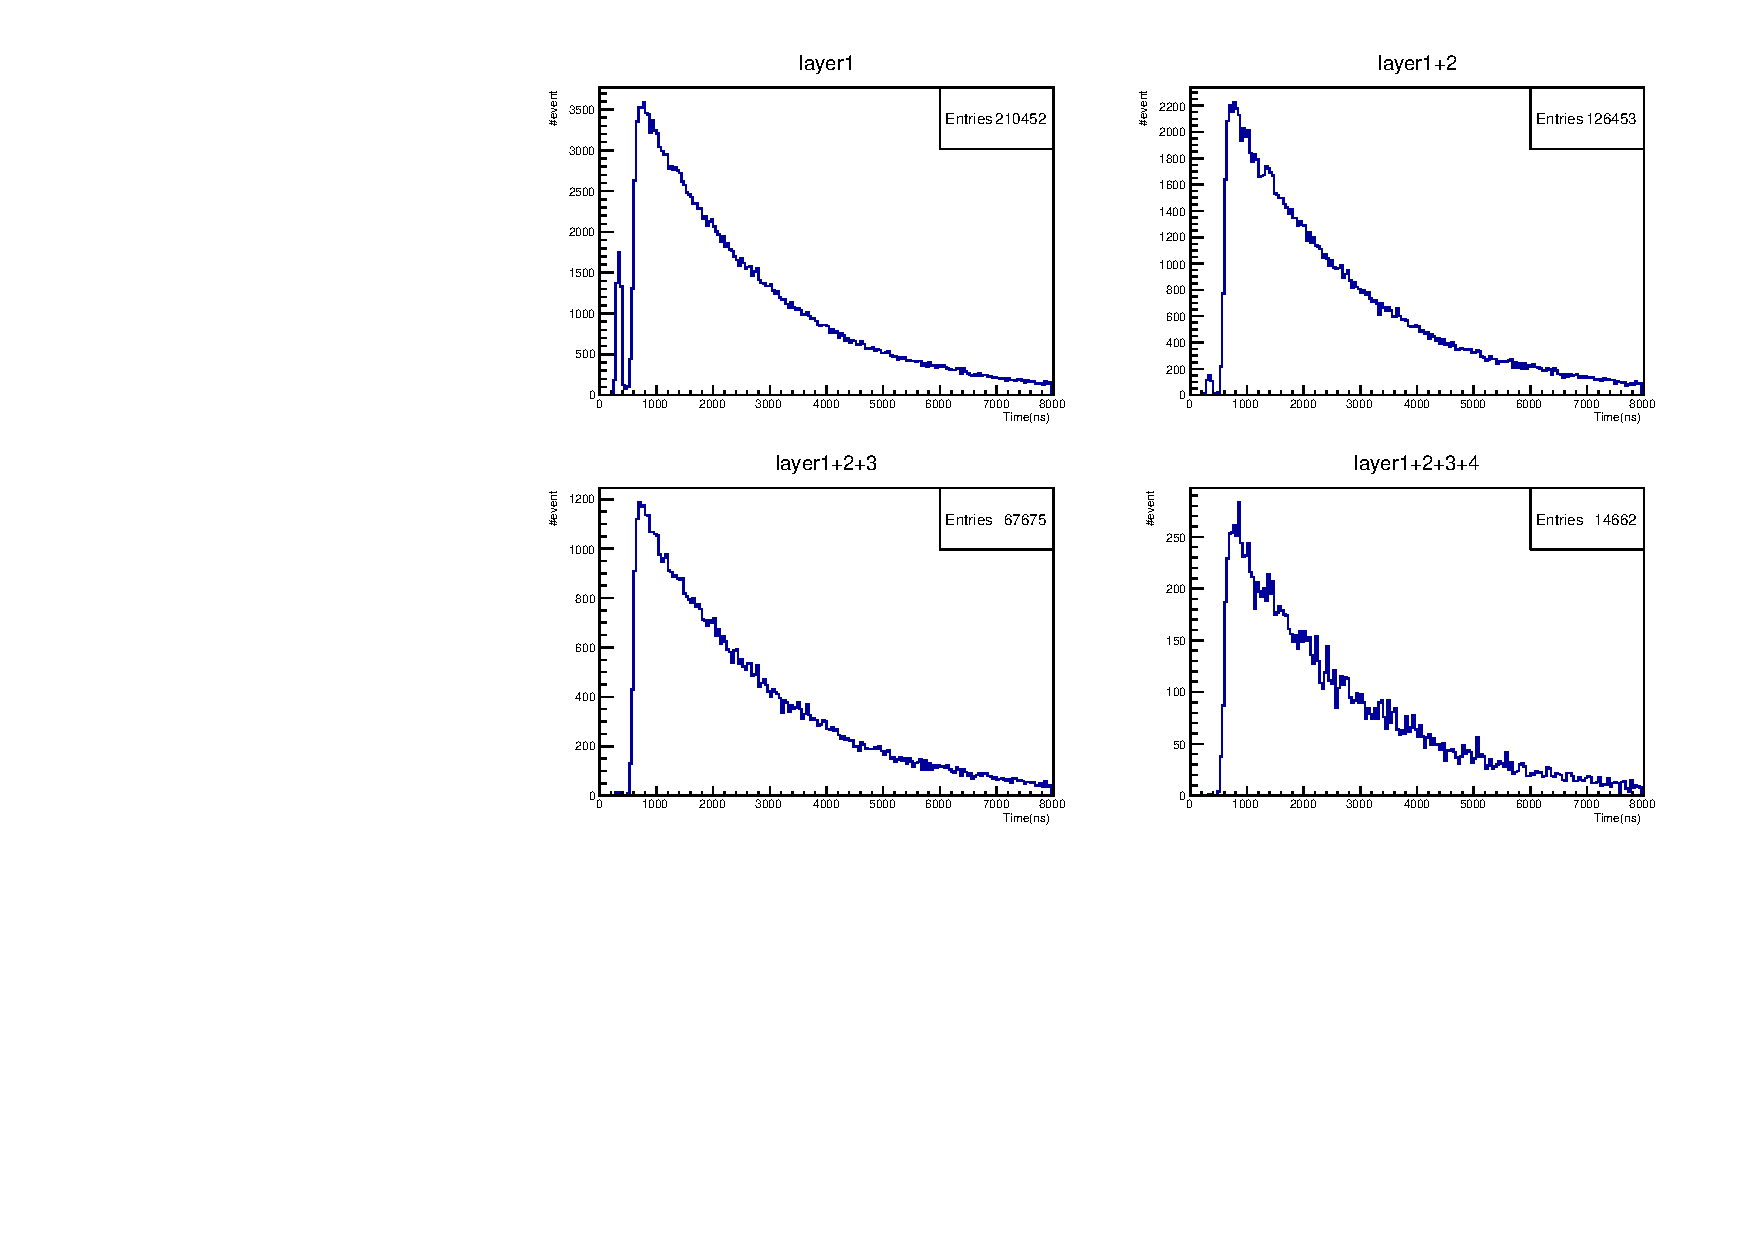
\includegraphics[height = 0.9\columnwidth , angle = -90]{figure/ikemitsu/lt_layercoin.pdf}
\caption{層でcoincidenceを取って得られたヒストグラム(磁場なし標的)}
\label{lt_layercoin}
\end{subfigure}
\begin{subfigure}{\columnwidth}
\centering
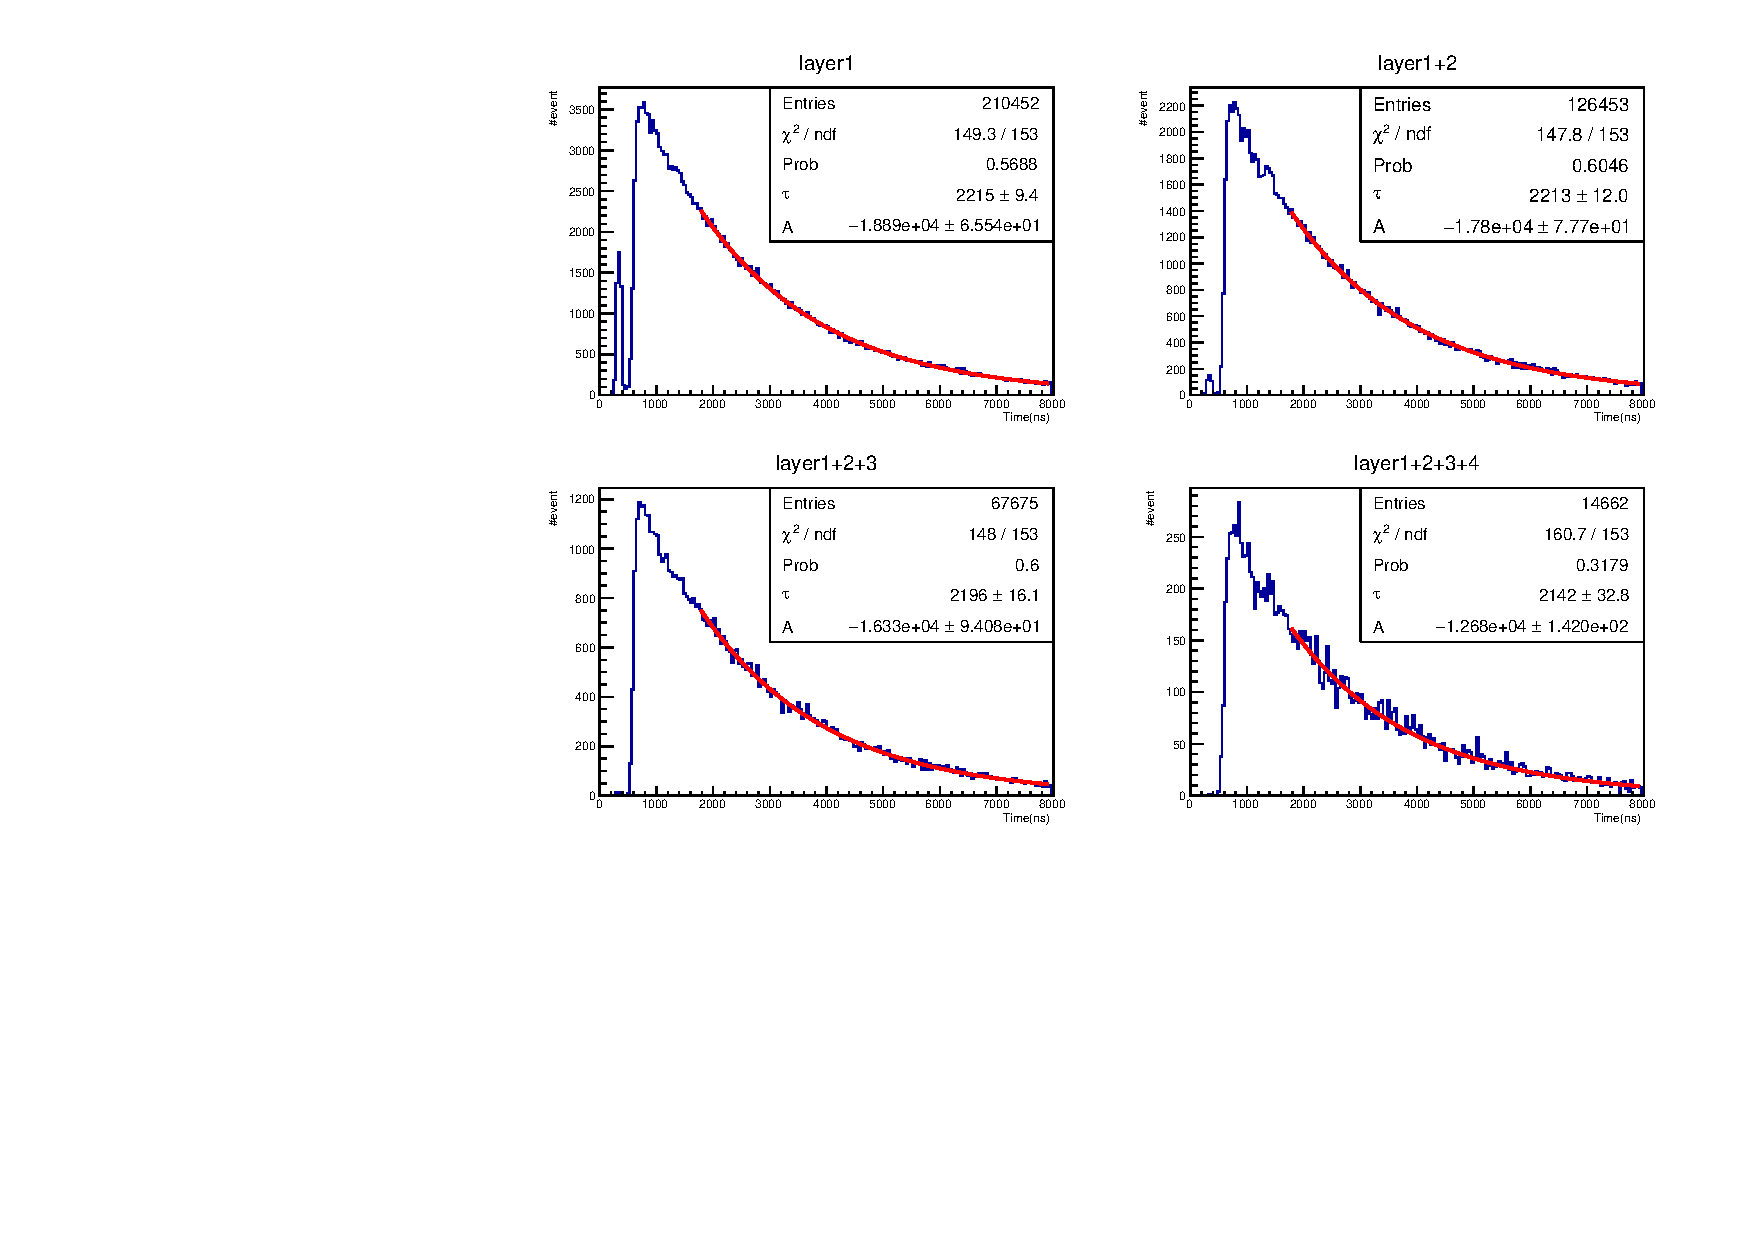
\includegraphics[height = 0.9\columnwidth , angle = -90]{figure/ikemitsu/lt_layercoin_fit.pdf}
\caption{$f_{\mathrm{life}}(t)$でfittingをした図}
\label{lt_layercoin_fit}
\end{subfigure}
\caption{fittingした図}
\label{lt_layercoin_all}
\end{figure}

\begin{figure}[H]
\centering
\begin{subfigure}{\columnwidth}
\centering
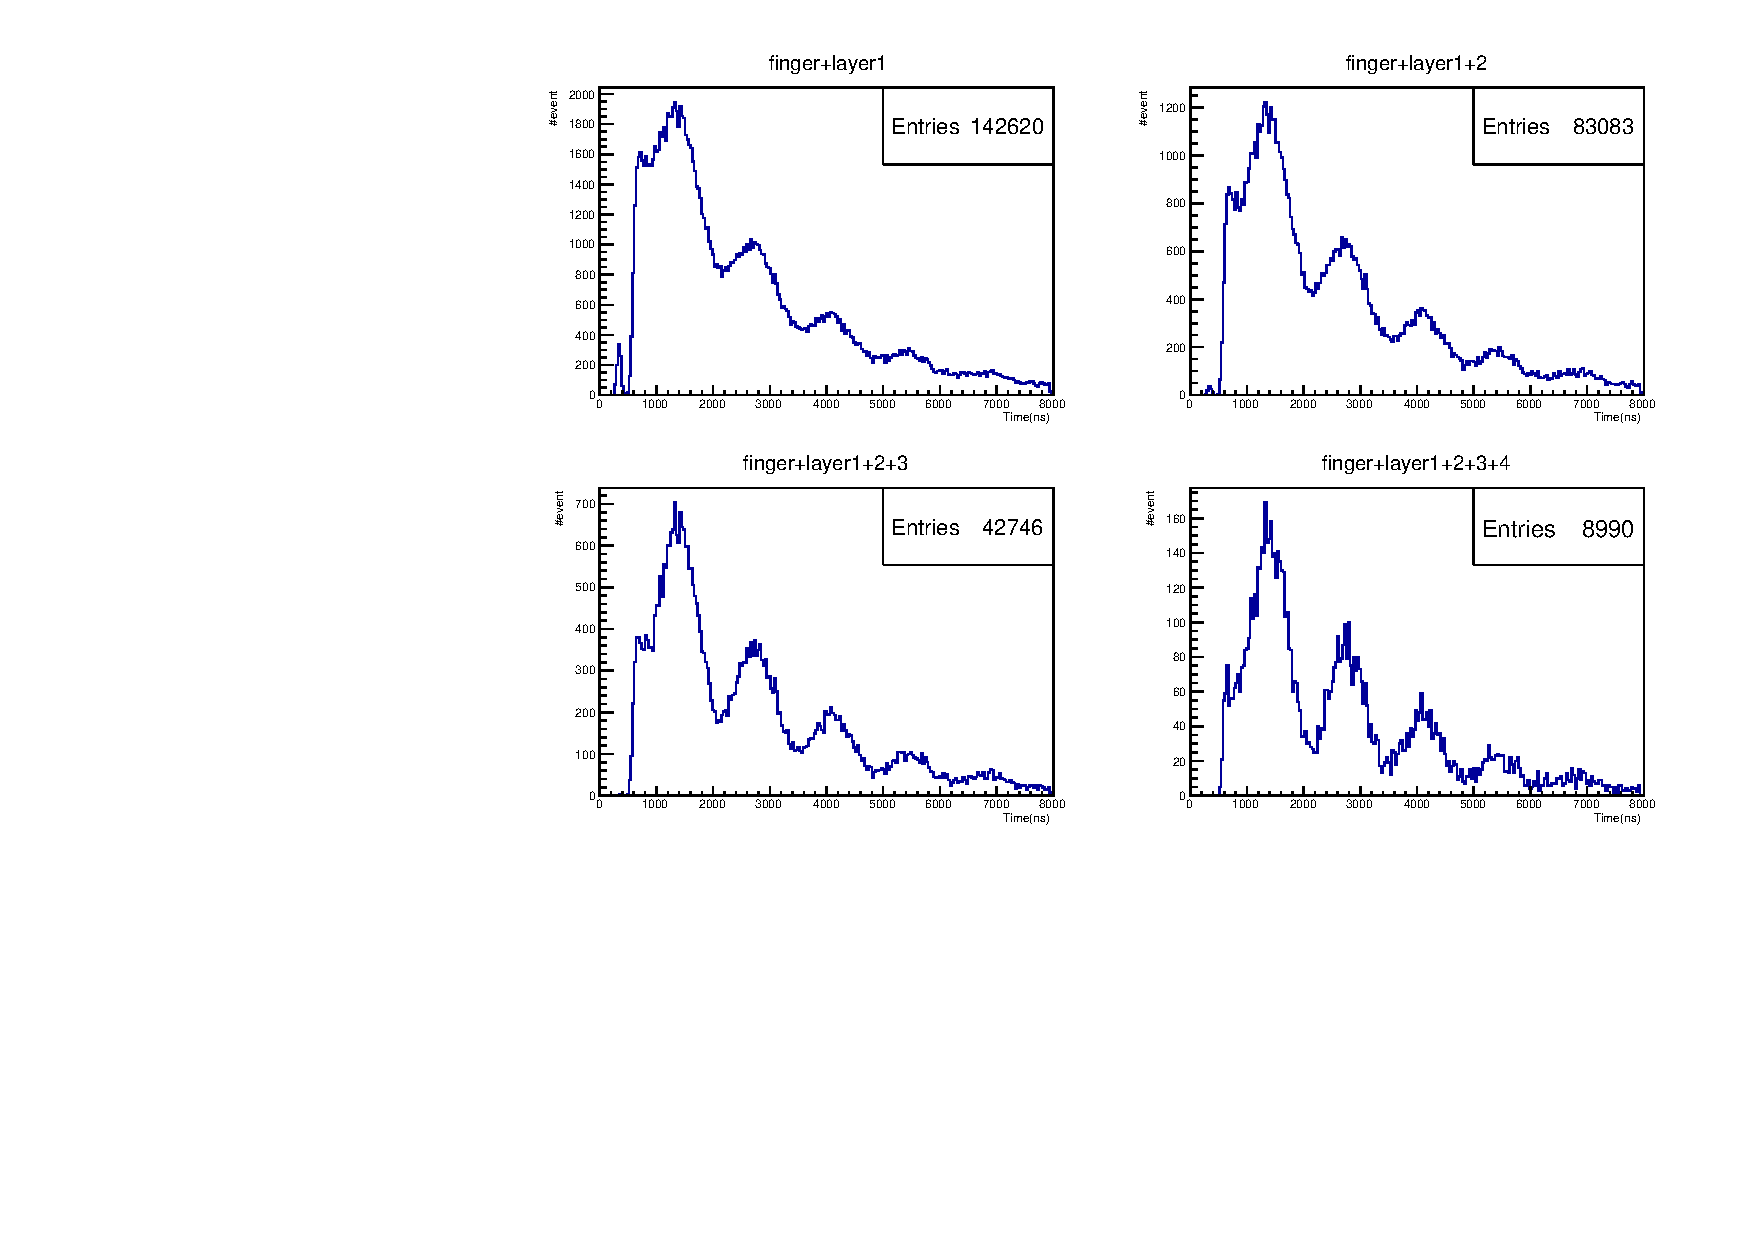
\includegraphics[height = 0.9\columnwidth , angle = -90]{figure/ikemitsu/g_layer_f_coin.pdf}
\caption{層でcoincidenceを取って得られたヒストグラム(磁場あり標的)}
\label{g_layercoin}
\end{subfigure}
\begin{subfigure}{\columnwidth}
\centering
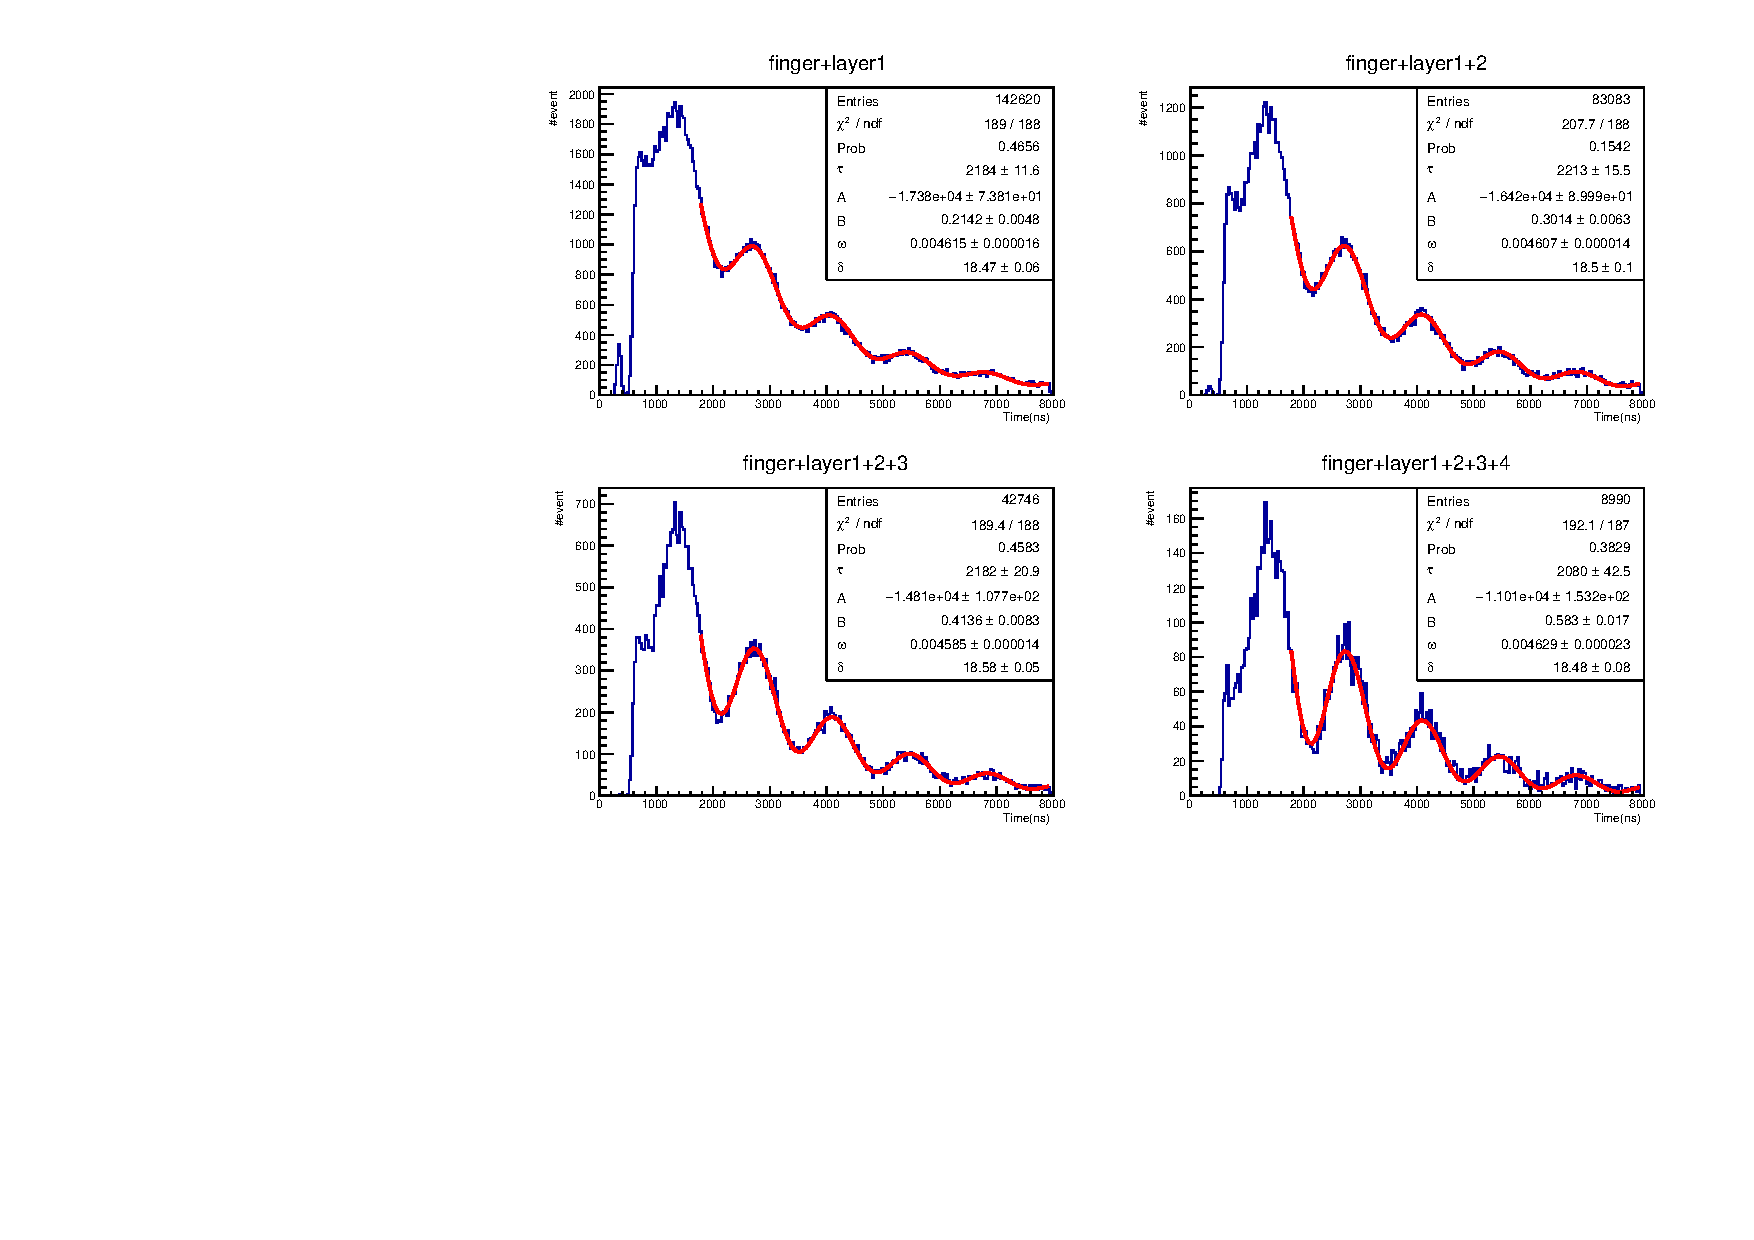
\includegraphics[height = 0.9\columnwidth , angle = -90]{figure/ikemitsu/g_laye_f_coin_fit.pdf}
\caption{$f_{g}(t)$でfittingをした図}
\label{g_layercoin_fit}
\end{subfigure}
\caption{fittingした図}
\label{g_layercoin_all}
\end{figure}

\subsubsection{エネルギー分布}
磁場なし標的を用いたときのデータから求めたエネルギー分布は図\ref{michel_PS}のようになった.
さらに,図\ref{michel_PS}の各点において,キャリブレーションに由来するエネルギー分解能と統計誤差をそれぞれ横軸と縦軸の誤差として付けたのが図\ref{michel_PS_gosa}である.
\begin{figure}[H]
\centering
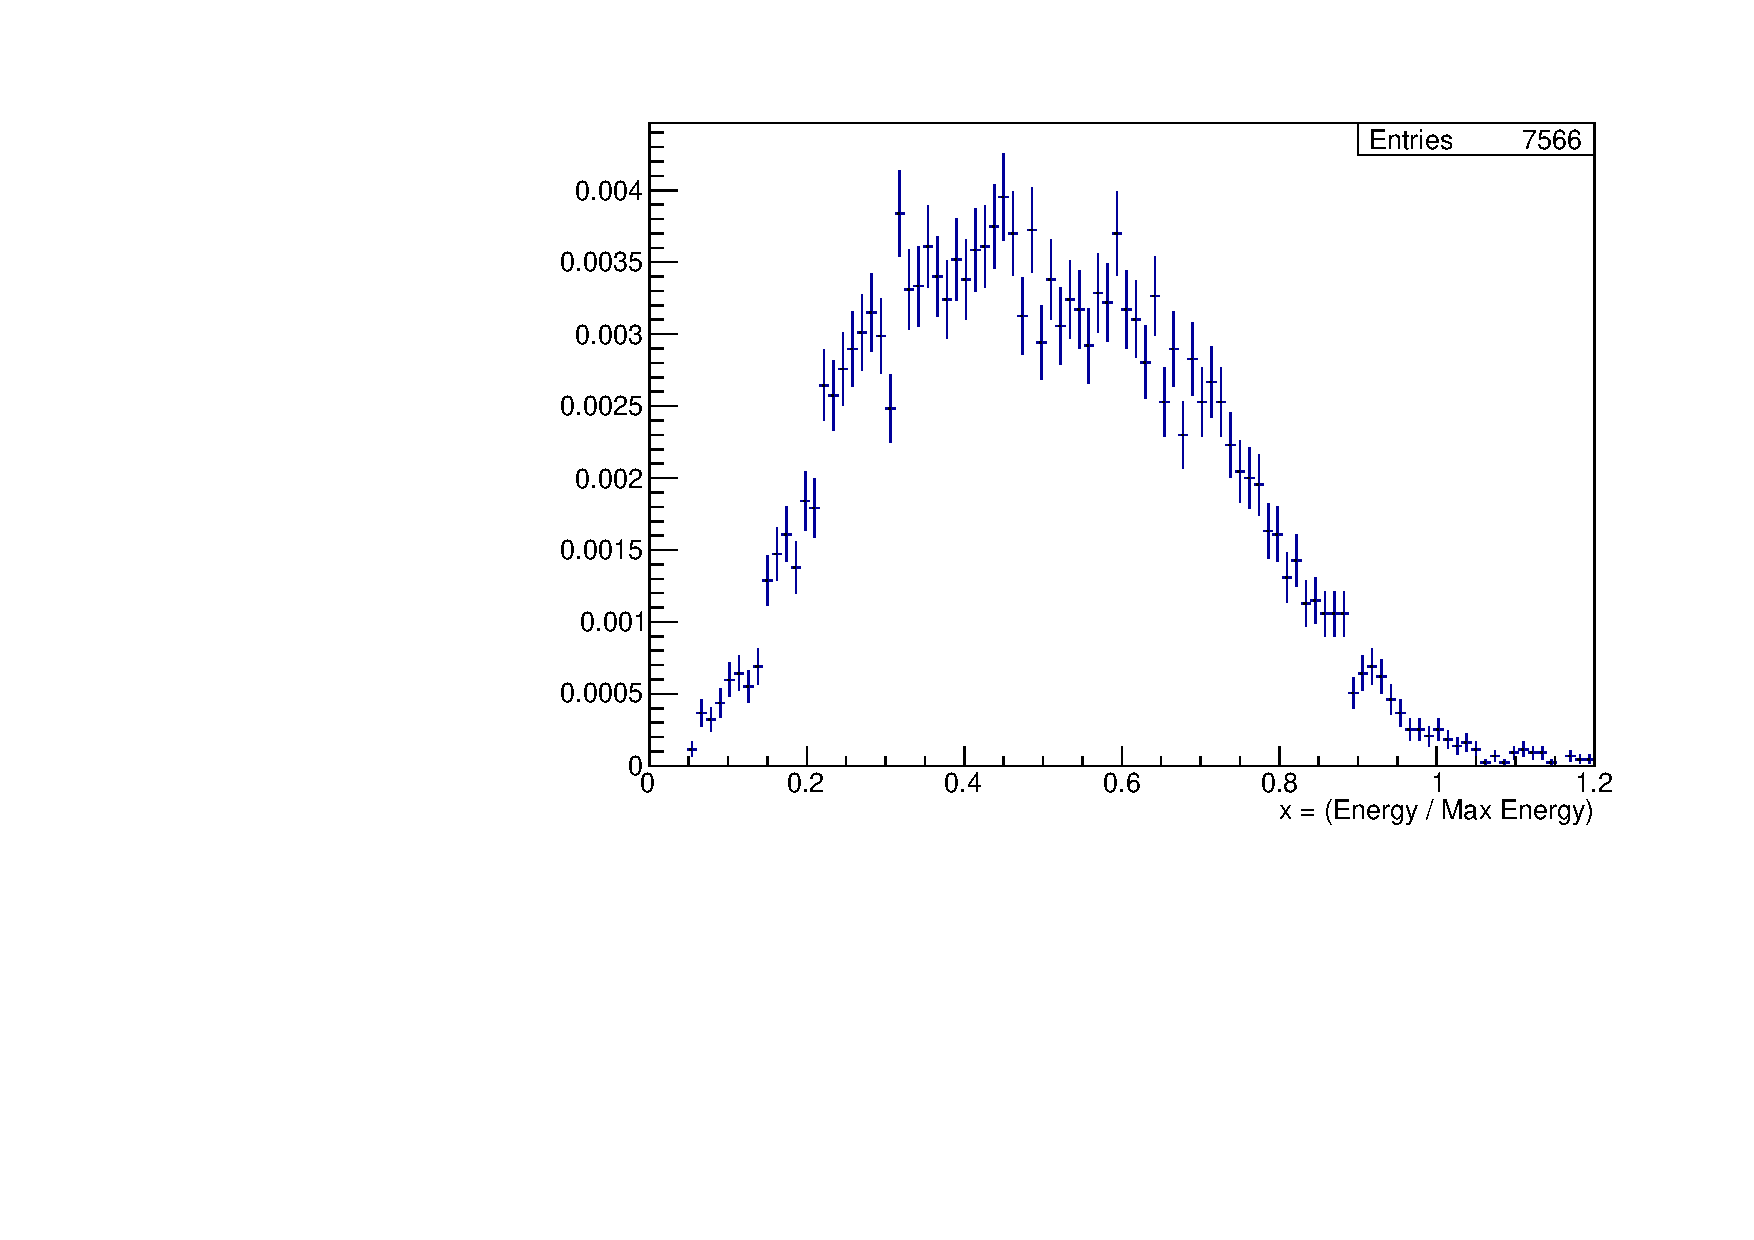
\includegraphics[height = 0.7\columnwidth , angle = -90]{figure/ikemitsu/michel_PS.pdf}
\caption{PSで得られたエネルギー分布図;磁場なし標的}
\label{michel_PS}
\end{figure}

\begin{figure}[H]
\centering
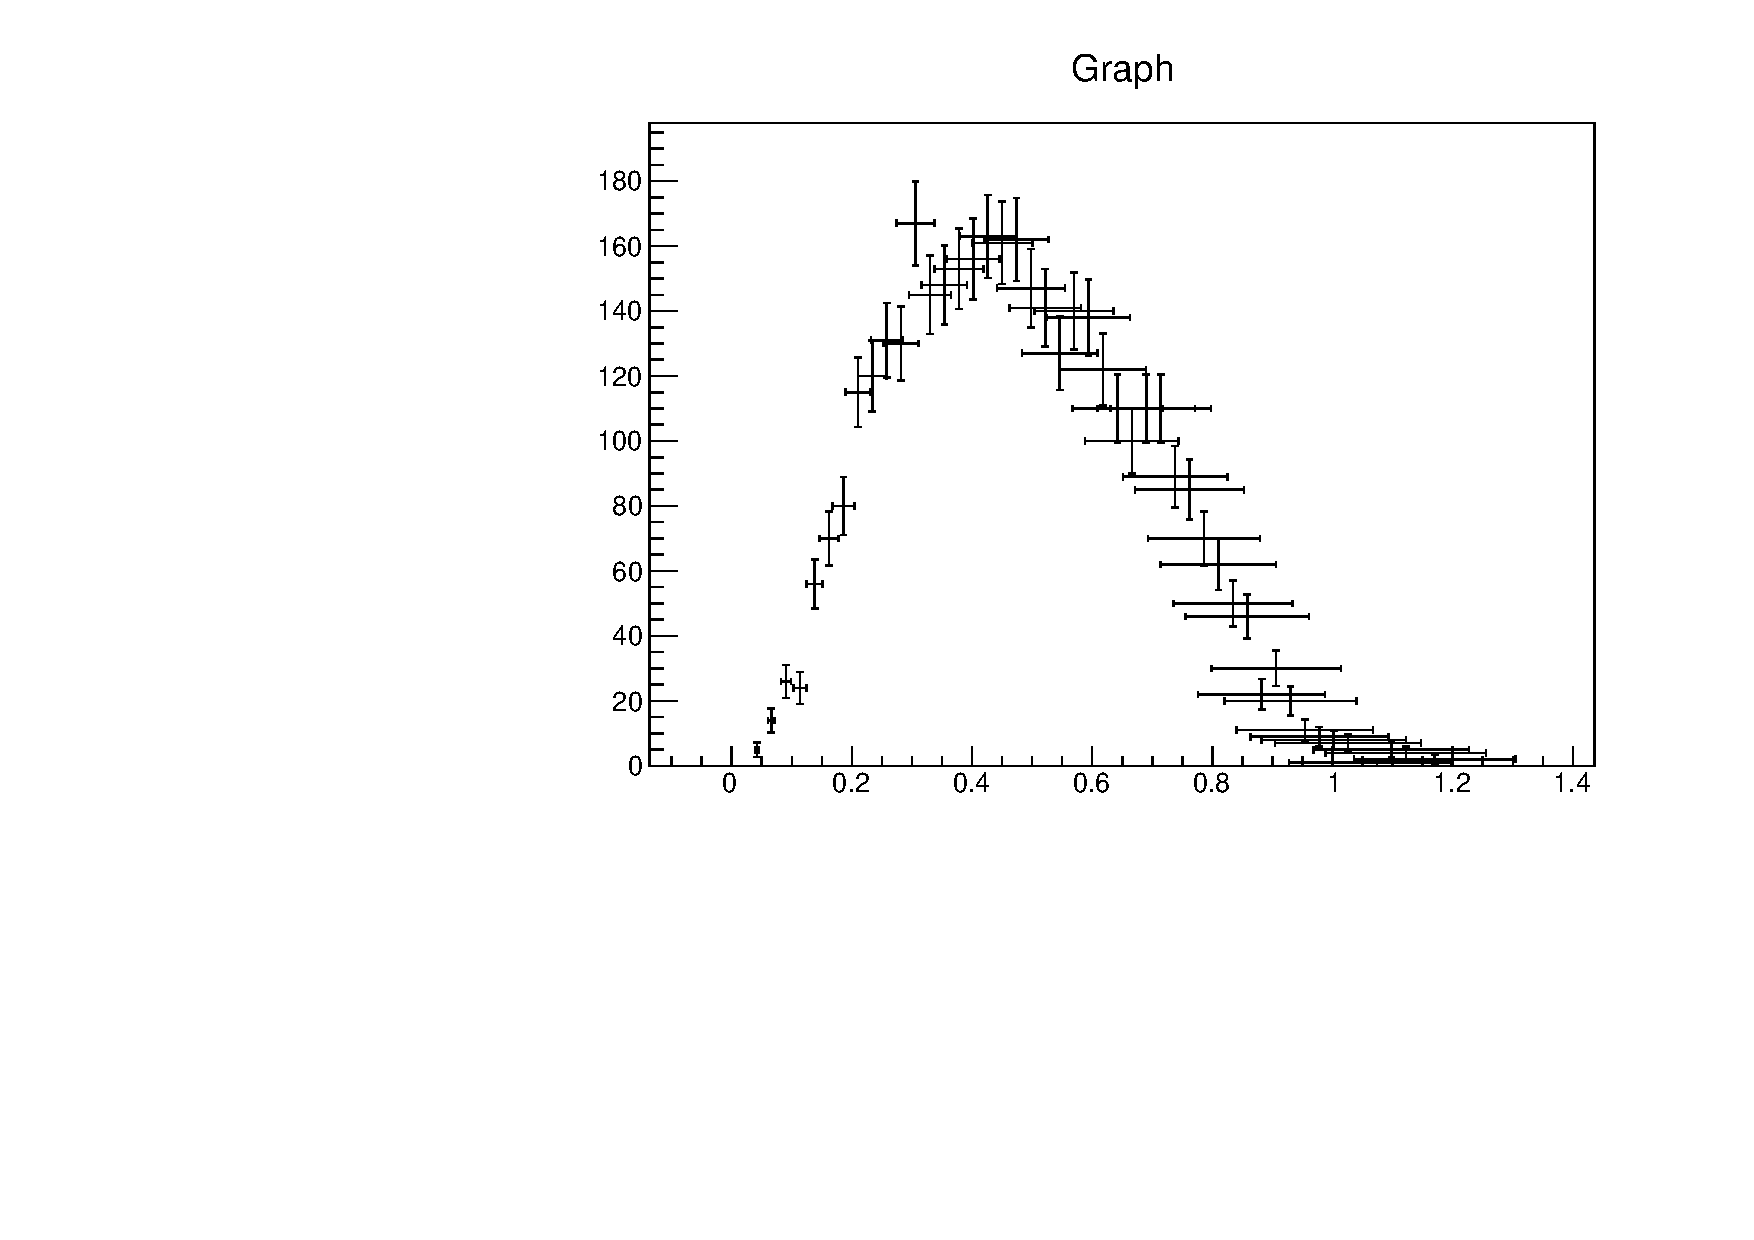
\includegraphics[height = 0.7\columnwidth , angle = -90]{figure/ikemitsu/michel_PS_gosa.pdf}
\caption{PSで得られたエネルギー分布(誤差付き);磁場なし標的}
\label{michel_PS_gosa}
\end{figure}

ミュオンのスピンに対して角度$\theta$の方向に崩壊する$\mathrm{e}^{+}$のエネルギー分布は,式\ref{eq:theory_michel}で与えられた.
この式に$\rho$以外のパラメータの値として,標準模型で予想されている$\eta = 0 , \xi = 1 , \xi \delta = 3/4$を代入して計算すると,
\begin{equation*}
\frac{d\Gamma}{dx} \propto x^{2} [\frac{2}{3}(\rho + \frac{3}{8}\cos \theta - \frac{1}{8})(4x-3) + \frac{1}{4}(\cos \theta + 3)]
\end{equation*}
となる.

図\ref{michel_PS_gosa}のグラフを$f_{\mathrm{michel}}(x) = x^{2} (A(4x -3) + B)$でfittingすることにより$\rho$を求めることができると考えた.
しかし,高エネルギー側での横軸の誤差が大きいこともありfittingはうまくいかなかった.以下ではエネルギー解析についての課題を述べる.

プラスチックシンチレータは無機シンチレータに比べて密度が小さいので,電磁シャワーで生じたフォトンが検出器の外側に漏れやすい.
これによって高エネルギーの粒子の観測数が減ると考えられる.
解析的にこの課題を解決するには,シミュレーションによって入射粒子のエネルギーと観測されるエネルギーの対応を求めてfitting関数にその寄与を組み込む必要がある.

また,この実験ではPSのエネルギー較正に改善の余地が大いに残されている.
宇宙線ミュオンを用いたキャリブレーションならば,NaI検出器で行っているような,fingerとのcoincidenceをとることで精度を上げることができると考えられる.

\subsubsection{fitting範囲による寿命と$g$因子の系統誤差}
今回使用したミュオンビームの分布は,FWHM$\sim$100 ns の幅を持ったガウス分布である.
よって,図\ref{lt_layercoin}のヒストグラムのピーク点は750 ns であるが,その点から1000 ns はfittingの対象外とし,
図\ref{lt_layercoin_fit}と図\ref{g_layercoin_fit}ではfittingの範囲を1750 ns から7950 ns までとした.

この範囲の前側と後側で範囲を分けてfittingをすると,$\tau$と$g$の値は表\ref{fitrange1}〜\ref{fitrange4}のようになった.
\begin{table}[H]
\caption{$\tau$;fitting範囲1750 ns 〜5250 ns}
\label{fitrange1}
\begin{center}
\begin{tabular}{cc}\toprule
coincidenceを取った層 	& $\tau$(ns) \\ \midrule
1 			& 2197 $\pm$ 16 \\
1+2 			& 2189 $\pm$ 20 \\
1+2+3 			& 2200 $\pm$ 28 \\
1+2+3+4 		& 2211 $\pm$ 60 \\ \bottomrule
\end{tabular}
\end{center}
\end{table}%

\begin{table}[H]
\caption{$\tau$;fitting範囲4450 ns 〜7950 ns}
\label{fitrange2}
\begin{center}
\begin{tabular}{cc}\toprule
coincidenceを取った層 	& $\tau$(ns) \\ \midrule
1 			& 2247 $\pm$ 30 \\
1+2 			& 2244 $\pm$ 37 \\
1+2+3 			& 2218 $\pm$ 50 \\
1+2+3+4 		& 2036 $\pm$ 91 \\ \bottomrule
\end{tabular}
\end{center}
\end{table}%

\begin{table}[H]
\caption{$g$;fitting範囲1750 ns 〜5250 ns}
\label{fitrange3}
\begin{center}
\begin{tabular}{ccc}\toprule
coincidenceを取った層 	& $\omega$(/ns) 			& $g$ \\ \midrule
finger+1 		& $( 4.608 \pm 0.025 ) \times 10^{-3}$ 	& 2.004  $\pm$ 0.011 \\
finger+1+2 		& $( 4.585 \pm 0.023 ) \times 10^{-3}$ 	& 1.9938 $\pm$ 0.0098 \\
finger+1+2+3 		& $( 4.576 \pm 0.022 ) \times 10^{-3}$ 	& 1.9896 $\pm$ 0.0095 \\
finger+1+2+3+4 		& $( 4.615 \pm 0.032 ) \times 10^{-3}$ 	& 2.007  $\pm$ 0.014 \\ \bottomrule
\end{tabular}
\end{center}
\end{table}%

\begin{table}[H]
\caption{$g$;fitting範囲4450 ns 〜7950 ns}
\label{fitrange4}
\begin{center}
\begin{tabular}{ccc}\toprule
coincidenceを取った層 	& $\omega$(/ns) 			& $g$ \\ \midrule
finger+1 		& $( 4.570 \pm 0.060 ) \times 10^{-3}$ 	& 1.987 $\pm$ 0.024 \\
finger+1+2 		& $( 4.589 \pm 0.049 ) \times 10^{-3}$ 	& 1.995 $\pm$ 0.021 \\
finger+1+2+3 		& $( 4.579 \pm 0.049 ) \times 10^{-3}$ 	& 1.991 $\pm$ 0.021 \\
finger+1+2+3+4 		& $( 4.607 \pm 0.091 ) \times 10^{-3}$ 	& 2.003 $\pm$ 0.040 \\ \bottomrule
\end{tabular}
\end{center}
\end{table}%

これらの結果を表\ref{fit_lt}・表\ref{fit_g}と比較すると,fittingの範囲を変えても,得られた$\tau$と$g$の値は誤差の範囲内で一致していると言える.
このことから,fittingの範囲として1750 ns から7950 ns までは適切だと考えられる.

しかし,寿命に関して,表\ref{fitrange1}と表\ref{fitrange2}の1,2段目を比較すると,遅い時間側でfittingを行うと寿命が長くなっていると分かる.
これは,バックグラウンドなどのノイズを信号として処理しており,その影響がイベント数の少ない部分で強く出ていることによると考えることができる.
これを除くためには,より詳しい波形解析によってノイズとみなせる信号の性質を特定しなければならない.
今回の実験ではバックグラウンド計測をしなかったが,今後の課題として,ノイズ除去を目的とした解析を行う必要がある.
FADCを用いた実験では波形をデータとして残せるので,ノイズに起因する信号を取り除くことは可能だと考えられる.
寿命の解析結果として,表\ref{fit_lt}と表\ref{fitrange1}・表\ref{fitrange2}の違いをfitting範囲による系統誤差に含めた.

$g$因子については,バックグラウンドがあっても振動の周期への影響はないと考えられる.
したがって,fitting範囲による系統誤差はないとした.

\subsubsection{この節のまとめ}
解析の結果得られたミュオンの寿命と$g$因子の値は表\ref{matome_ike}のようになった.寿命の誤差は統計誤差とfitting範囲による系統誤差で,$g$因子の誤差は統計誤差である.

\begin{table}[H]
\caption{解析結果}
\label{matome_ike}
\begin{center}
\begin{tabular}{cc}\toprule
$\tau$(ns) 	& 2212 $\pm$ 12 $^{ + 35}_{ - 15}$  \\ \midrule
$g$		& 2.003 $\pm$ 0.006 \\ \bottomrule
\end{tabular}
\end{center}
\end{table}%

%%%%%%%%%%%%%%%%%%%池満パート終了%%%%%%%%%%%%%%%%%%%

%\end{document}
